% Copyright (c) 2017-2020 Matematyka dla Ciekawych Świata (http://ciekawi.icm.edu.pl/)
% Copyright (c) 2017-2020 Robert Ryszard Paciorek <rrp@opcode.eu.org>
% Copyright (c) 2020 Krzysztof Lasocki <krz.lasocki@gmail.com>
% 
% MIT License
% 
% Permission is hereby granted, free of charge, to any person obtaining a copy
% of this software and associated documentation files (the "Software"), to deal
% in the Software without restriction, including without limitation the rights
% to use, copy, modify, merge, publish, distribute, sublicense, and/or sell
% copies of the Software, and to permit persons to whom the Software is
% furnished to do so, subject to the following conditions:
% 
% The above copyright notice and this permission notice shall be included in all
% copies or substantial portions of the Software.
% 
% THE SOFTWARE IS PROVIDED "AS IS", WITHOUT WARRANTY OF ANY KIND, EXPRESS OR
% IMPLIED, INCLUDING BUT NOT LIMITED TO THE WARRANTIES OF MERCHANTABILITY,
% FITNESS FOR A PARTICULAR PURPOSE AND NONINFRINGEMENT. IN NO EVENT SHALL THE
% AUTHORS OR COPYRIGHT HOLDERS BE LIABLE FOR ANY CLAIM, DAMAGES OR OTHER
% LIABILITY, WHETHER IN AN ACTION OF CONTRACT, TORT OR OTHERWISE, ARISING FROM,
% OUT OF OR IN CONNECTION WITH THE SOFTWARE OR THE USE OR OTHER DEALINGS IN THE
% SOFTWARE.

\section{Przygotowanie mikrokontrolera STM32}

Bardzo możliwe, że Twój mikrokontroler nie będzie miał przylutowanych pinów do połączenia z płytką stykową.
W takim wypadku będziesz musiał/musiała użyć lutownicy, aby je przylutować.\\

\begin{ProTip}{\normalfont{\strong{Ostrożnie}}}
  Podczas pracy, grot (metalowa końcówka) lutownicy jest rozgrzany do 200-400 stopni Celsjusza. Zachowaj ostrożność
  podczas jej używania. Zapamiętaj:
  \begin{itemize}
  \item Zawsze odkładaj lutownicę do stojaka. Nigdy nie kładź jej luzem na stole.
  \item Nigdy nie łap za metalowy koniec lutownicy.
  \item Nie wolno łapać spadającej lutownicy. Nie martw się, zawszę można kupić nową.
  \item Grot lutownicy jest gorący przez jakiś czas po wyłączeniu.
  \item Nie zostawiaj włączonej lutownicy bez opieki.
  \item \textbf{Przed lutowaniem musisz odłączyć układ (lub urządzenie) od zasilania}.
  \end{itemize}
\end{ProTip}

Do lutowania drobnej elektroniki (takiej jak mikrokontrolery i układy scalone) najepsza jest precyzyjna lutownica o małej mocy (do 30W),
z regualcją temperatury oraz ostrym lub małym płaskim (w kształcie śrubokręta płaskiego, około 2mm szerokości) grotem. Potrzebny jest też do niej
stojak. Inne przydatne akcesoria to kalafonia (ułatwia lutowanie) lub topnik (elektroniczny), oraz wyciorek do wycierania grotu - może być to specjalna gąbka (zwilżona
przed użyciem) lub druciak do mycia naczyń.\\

Najwygodniej jest używać spoiwo lutownicze w formie drutu o średnicy nie większej niż 0.5 mm, najlepiej 0.25mm. Przy budowie prototypów
najczęściej używa się cyny ołowiowej Sn40/Pb60 (stop 40\% cyny oraz 60\% ołowiu).
\\

\begin{figure}[h!]\begin{Ramka}{}\begin{center}
  {\noindent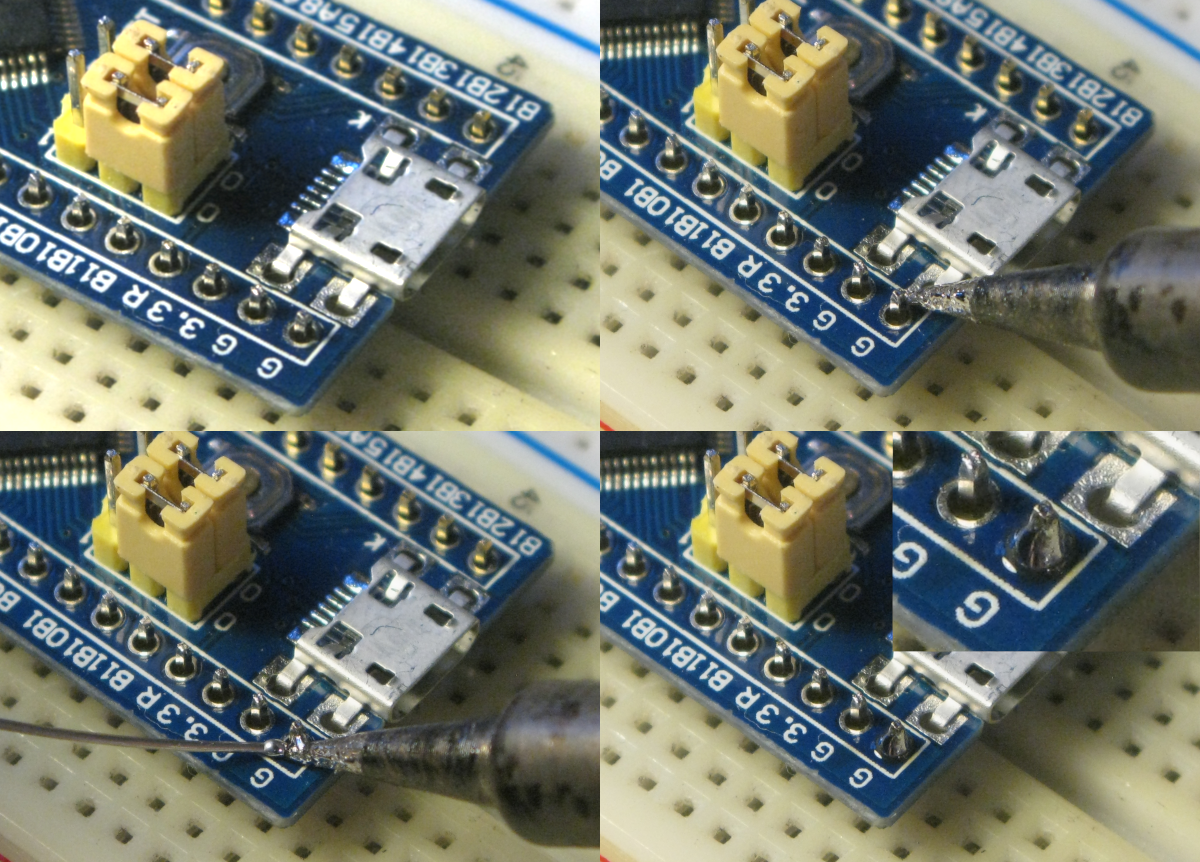
\includegraphics[width=0.99\textwidth,clip=true]{warsztat_elektroniczny/lutowanie}}\\
  \small
  \textbf{Lutowanie pinu mikrokontrolera.} Listwy kołkowe zostały umieszczone w płytce stykowej, aby je umiejscowić. \textit{Zaczynając od lewego górnego zdjęcia,
    zgodnie z ruchem wskazówek zegara:} Umiejscowienie pinu. Ogrzanie pinu i pola lutowniczego na płytce mikrokontrolera.
  Dotknięcie spoiwem (cyną).
  Gotowy lut (oraz jego przybliżenie).
\end{center}\end{Ramka}\end{figure}

Jeżeli Twój mikrokontroler nie ma przylutowanych pinów, musisz przylutować je sam/sama. Przymierz i odetnij
obcążkami dwa odcinki listwy kołkowej pasujące do otworów na brzegach płytki mikrokontrolera. Włóż piny do otworków
na płytce. Następnie odwiń lub wyciągnij odcinek cyny ze szpulki. Włącz lutownicę i odłóż ją na stojak. Jeżeli twoja lutownica
ma ustawianie temperatury, ustaw ją na około 250-300 st. C. Daj jej około minuty na osiągnięcie temperatury. Pamiętaj, że grot
lutownicy jest bardzo gorący. Lutownicę należy trzymać tylko i wyłącznie za rękojeść.
\\

Aby zalutować pin w otworze, najpierw dotknij grotem lutownicy
miejsca, które będziesz lutować (pola lutowniczego) oraz pinu. Trzeba ogrzać oba elementy przed ich połączeniem. Po około sekundzie, dotknij pinu końcówką odcinka cyny.
\\

Postaraj się, aby listwy kołkowe były prostopadle do płytki. Jeżeli masz odcinek damskiej listwy, możesz za jego pomocą
umiejscowić piny, które lutujesz. Możesz też użyć do tego płytki stykowej. Lutowanie zacznij od czterech pinów na rogach płytki.
\\

Kształt gotowego lutu powinien być stożkowaty. Jeżeli jest obły, oznacza to zbyt dużą ilość użytej cyny. Kuliste luty prawdopodobnie nie związały pinu z płytką (pole lutownicze nie było dobrze ogrzane). Jeśli lut nie jest błyszczący, oznacza to, że niepoprawnie związał (tzw. \textit{zimny lut}). W takim wypadku spróbuj dodać
topnika (np. kalafonii).\\

Umiejętne lutowanie wymaga trochę praktyki, ale nie jest skomplikowane. Pamiętaj, aby lutować w dobrze wentylowanym
pomieszczeniu. Po zakończeniu umyj ręce.
